\subsection{Contrôle live dans Escape}
\begin{figure}[htbp]
  \centering
  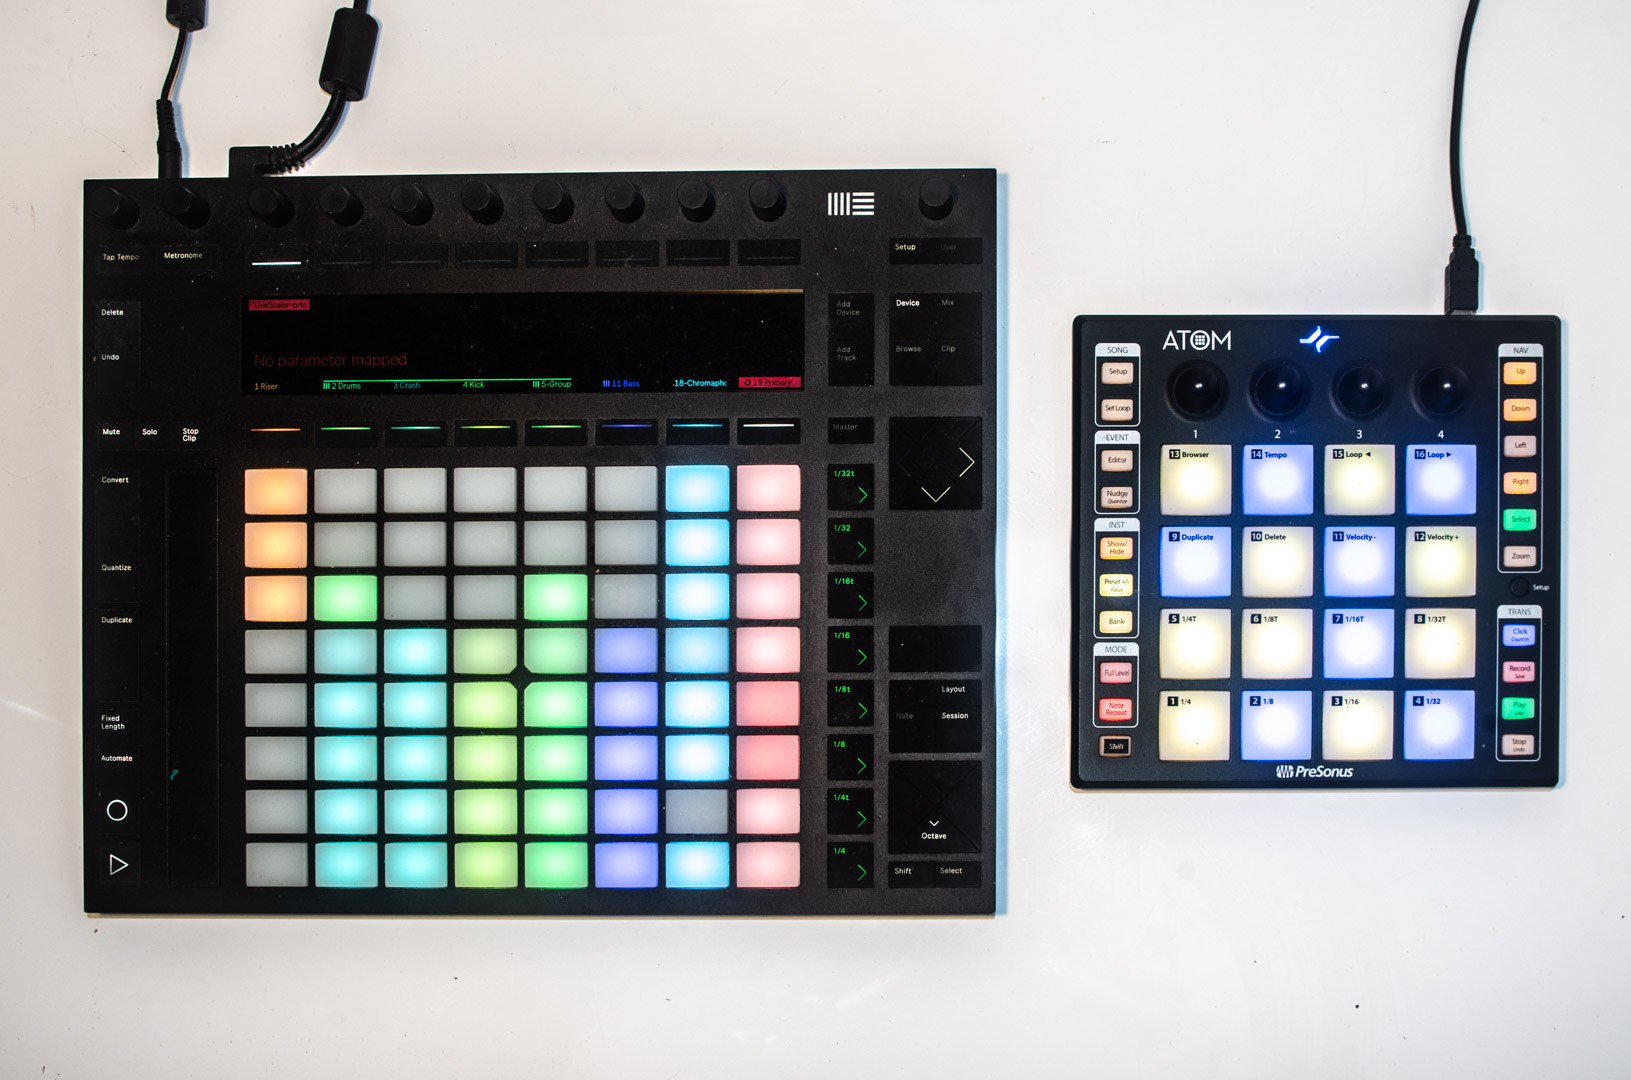
\includegraphics[width=\textwidth]{Figures/IMGP9899.jpg}
  \caption{Contrôleurs MIDI utilisés pour la performance live : à gauche le Push 2 par Ableton (contrôle de la structure du morceau) et à droite ATOM par Presonus (contrôle de l'harmonie du morceau).\label{fig:controleurs}}
\end{figure}
Pour \emph{Escape}, j'utilise deux contrôleurs MIDI distincts (voir Figure \ref{fig:controleurs}) :
\begin{itemize}
  \item le Push 2 par Ableton, qui est conçu spécialement pour contrôler Ableton Live. Il me permet de recréer en live la structure d'Escape en déclenchant ses différentes parties.
  \item l'ATOM de Presonus, composé d'une grille de$4\times 4$ touches qui me permettent de déclencher les transformations de gamme de \emph{LiveScaler}.
\end{itemize}

La figure \ref{fig:mapping-ATOM} illustre la manière (le plus souvent appelée \emph{mapping}) dont les touches de l'ATOM sont associées à des transformations de LiveScaler




